%% Elsevier "Internet of Things" (ISSN 2542-6605) submission.
%% Double-column final-submission layout (LaTeX-only per journal guide).
%% Build in the rl-iot-thesis container (has elsarticle + elsarticle-num.bst).
\documentclass[3p,twocolumn]{elsarticle}

\usepackage[T1]{fontenc}
\usepackage[utf8]{inputenc}
\usepackage{lmodern}
\usepackage{amsmath,amssymb}
\usepackage{graphicx}
\usepackage{booktabs}
\usepackage{multirow}
\usepackage{array}
\usepackage{makecell}
\usepackage{url}
\usepackage{xcolor}
\usepackage{hyperref}
\hypersetup{colorlinks=true,linkcolor=black,citecolor=black,urlcolor=blue}

\graphicspath{{figs/}}

%% Macro-driven numbers regenerated from docs/results/ via `make render-tables`.
%% Copied into paper/ so the manuscript builds standalone in the container.
% Auto-generated from docs/results/ablation/Falpha_summary.json and docs/results/ablation/Fcoupling_summary.json -- do not hand-edit.
% Regenerate with: PYTHONPATH=. .venv/bin/python -m scripts.thesis.render_tables
\newcommand{\NumSeeds}{10}
\newcommand{\AlphaZeroPPO}{+138.6}
\newcommand{\AlphaZeroPPOCILow}{+129.0}
\newcommand{\AlphaZeroPPOCIHigh}{+147.7}
\newcommand{\AlphaZeroDQN}{+116.6}
\newcommand{\AlphaZeroDQNCILow}{+102.6}
\newcommand{\AlphaZeroDQNCIHigh}{+130.7}
\newcommand{\AlphaZeroATwoC}{+147.1}
\newcommand{\AlphaZeroATwoCCILow}{+137.9}
\newcommand{\AlphaZeroATwoCCIHigh}{+156.2}
\newcommand{\AlphaZeroRF}{+136.5}
\newcommand{\AlphaZeroOracle}{+194.8}
\newcommand{\AlphaZeroGap}{+2.1}
\newcommand{\AlphaZeroVerdict}{overlapping}
\newcommand{\AlphaTwoPPO}{+121.6}
\newcommand{\AlphaTwoPPOCILow}{+109.1}
\newcommand{\AlphaTwoPPOCIHigh}{+133.2}
\newcommand{\AlphaTwoDQN}{+83.1}
\newcommand{\AlphaTwoDQNCILow}{+64.5}
\newcommand{\AlphaTwoDQNCIHigh}{+99.1}
\newcommand{\AlphaTwoATwoC}{+153.6}
\newcommand{\AlphaTwoATwoCCILow}{+145.4}
\newcommand{\AlphaTwoATwoCCIHigh}{+161.4}
\newcommand{\AlphaTwoRF}{+113.2}
\newcommand{\AlphaTwoOracle}{+194.8}
\newcommand{\AlphaTwoGap}{+8.4}
\newcommand{\AlphaTwoVerdict}{overlapping}
\newcommand{\AlphaFourPPO}{+121.3}
\newcommand{\AlphaFourPPOCILow}{+108.6}
\newcommand{\AlphaFourPPOCIHigh}{+133.1}
\newcommand{\AlphaFourDQN}{+72.5}
\newcommand{\AlphaFourDQNCILow}{+53.5}
\newcommand{\AlphaFourDQNCIHigh}{+90.0}
\newcommand{\AlphaFourATwoC}{+138.7}
\newcommand{\AlphaFourATwoCCILow}{+128.0}
\newcommand{\AlphaFourATwoCCIHigh}{+150.0}
\newcommand{\AlphaFourRF}{+94.4}
\newcommand{\AlphaFourOracle}{+194.8}
\newcommand{\AlphaFourGap}{+26.9}
\newcommand{\AlphaFourVerdict}{significant}
\newcommand{\AlphaSixPPO}{+113.3}
\newcommand{\AlphaSixPPOCILow}{+100.4}
\newcommand{\AlphaSixPPOCIHigh}{+126.1}
\newcommand{\AlphaSixDQN}{+77.4}
\newcommand{\AlphaSixDQNCILow}{+60.4}
\newcommand{\AlphaSixDQNCIHigh}{+93.0}
\newcommand{\AlphaSixATwoC}{+151.4}
\newcommand{\AlphaSixATwoCCILow}{+141.9}
\newcommand{\AlphaSixATwoCCIHigh}{+159.8}
\newcommand{\AlphaSixRF}{+64.0}
\newcommand{\AlphaSixOracle}{+194.8}
\newcommand{\AlphaSixGap}{+49.3}
\newcommand{\AlphaSixVerdict}{significant}
\newcommand{\AlphaEightPPO}{+135.2}
\newcommand{\AlphaEightPPOCILow}{+124.9}
\newcommand{\AlphaEightPPOCIHigh}{+145.1}
\newcommand{\AlphaEightDQN}{+75.7}
\newcommand{\AlphaEightDQNCILow}{+56.3}
\newcommand{\AlphaEightDQNCIHigh}{+93.0}
\newcommand{\AlphaEightATwoC}{+137.5}
\newcommand{\AlphaEightATwoCCILow}{+126.5}
\newcommand{\AlphaEightATwoCCIHigh}{+148.0}
\newcommand{\AlphaEightRF}{+20.5}
\newcommand{\AlphaEightOracle}{+194.8}
\newcommand{\AlphaEightGap}{+114.7}
\newcommand{\AlphaEightVerdict}{significant}
\newcommand{\AlphaOnePPO}{+131.9}
\newcommand{\AlphaOnePPOCILow}{+120.7}
\newcommand{\AlphaOnePPOCIHigh}{+141.9}
\newcommand{\AlphaOneDQN}{+67.6}
\newcommand{\AlphaOneDQNCILow}{+49.6}
\newcommand{\AlphaOneDQNCIHigh}{+85.0}
\newcommand{\AlphaOneATwoC}{+142.0}
\newcommand{\AlphaOneATwoCCILow}{+130.7}
\newcommand{\AlphaOneATwoCCIHigh}{+153.4}
\newcommand{\AlphaOneRF}{-29.3}
\newcommand{\AlphaOneOracle}{+194.8}
\newcommand{\AlphaOneGap}{+161.2}
\newcommand{\AlphaOneVerdict}{significant}
\newcommand{\HeadlineAlpha}{0.4}
\newcommand{\AnchorPPO}{+138.6}
\newcommand{\AnchorRF}{+136.5}
\newcommand{\OracleCeiling}{+194.8}
\newcommand{\CouplingGapCoupled}{-63.1}
\newcommand{\CouplingGapOutcome}{-63.0}
\newcommand{\CouplingBestCoupled}{DQN}
\newcommand{\CouplingBestOutcome}{A2C}
\newcommand{\CouplingDQNCoupled}{+226.2}
\newcommand{\CouplingPPOCoupled}{+162.4}
\newcommand{\CouplingATwoCCoupled}{+144.8}
\newcommand{\CouplingDQNOutcome}{-8.6}
\newcommand{\CouplingPPOOutcome}{+126.2}
\newcommand{\CouplingATwoCOutcome}{+146.1}
% --- F10 environment-difficulty sweep (PPO/A2C/DQN) ---
\newcommand{\FtenZeroPPO}{-46.2}
\newcommand{\FtenZeroPPOCILow}{-62.4}
\newcommand{\FtenZeroPPOCIHigh}{-32.2}
\newcommand{\FtenTwoPPO}{+5.1}
\newcommand{\FtenTwoPPOCILow}{-12.4}
\newcommand{\FtenTwoPPOCIHigh}{+23.0}
\newcommand{\FtenFourPPO}{+69.6}
\newcommand{\FtenFourPPOCILow}{+48.1}
\newcommand{\FtenFourPPOCIHigh}{+93.0}
\newcommand{\FtenSixPPO}{+90.9}
\newcommand{\FtenSixPPOCILow}{+74.0}
\newcommand{\FtenSixPPOCIHigh}{+107.0}
\newcommand{\FtenEightPPO}{+104.1}
\newcommand{\FtenEightPPOCILow}{+84.4}
\newcommand{\FtenEightPPOCIHigh}{+123.0}
\newcommand{\FtenOnePPO}{+142.6}
\newcommand{\FtenOnePPOCILow}{+132.6}
\newcommand{\FtenOnePPOCIHigh}{+152.2}
\newcommand{\FtenZeroDQN}{-79.6}
\newcommand{\FtenZeroDQNCILow}{-118.2}
\newcommand{\FtenZeroDQNCIHigh}{-43.1}
\newcommand{\FtenTwoDQN}{-36.8}
\newcommand{\FtenTwoDQNCILow}{-73.0}
\newcommand{\FtenTwoDQNCIHigh}{+0.7}
\newcommand{\FtenFourDQN}{-10.3}
\newcommand{\FtenFourDQNCILow}{-39.6}
\newcommand{\FtenFourDQNCIHigh}{+20.5}
\newcommand{\FtenSixDQN}{+44.6}
\newcommand{\FtenSixDQNCILow}{+10.4}
\newcommand{\FtenSixDQNCIHigh}{+82.3}
\newcommand{\FtenEightDQN}{+65.4}
\newcommand{\FtenEightDQNCILow}{+37.4}
\newcommand{\FtenEightDQNCIHigh}{+94.8}
\newcommand{\FtenOneDQN}{+78.3}
\newcommand{\FtenOneDQNCILow}{+41.8}
\newcommand{\FtenOneDQNCIHigh}{+110.3}
\newcommand{\FtenZeroATwoC}{-7.2}
\newcommand{\FtenZeroATwoCCILow}{-21.0}
\newcommand{\FtenZeroATwoCCIHigh}{+5.4}
\newcommand{\FtenTwoATwoC}{+25.9}
\newcommand{\FtenTwoATwoCCILow}{+18.1}
\newcommand{\FtenTwoATwoCCIHigh}{+33.2}
\newcommand{\FtenFourATwoC}{+72.8}
\newcommand{\FtenFourATwoCCILow}{+53.6}
\newcommand{\FtenFourATwoCCIHigh}{+88.0}
\newcommand{\FtenSixATwoC}{+101.5}
\newcommand{\FtenSixATwoCCILow}{+83.6}
\newcommand{\FtenSixATwoCCIHigh}{+116.7}
\newcommand{\FtenEightATwoC}{+123.0}
\newcommand{\FtenEightATwoCCILow}{+108.0}
\newcommand{\FtenEightATwoCCIHigh}{+139.0}
\newcommand{\FtenOneATwoC}{+147.3}
\newcommand{\FtenOneATwoCCILow}{+136.5}
\newcommand{\FtenOneATwoCCIHigh}{+156.5}
\newcommand{\FtenGSevenThreePPO}{Yes}
\newcommand{\FtenGSevenThreeDQN}{Yes}
\newcommand{\FtenGSevenThreeATwoC}{Yes}
% --- F17 evasion-before-commit sweep (PPO/A2C/DQN) ---
\newcommand{\FseventeenZeroReward}{+123.2}
\newcommand{\FseventeenZeroCompromise}{0.451}
\newcommand{\FseventeenTwentyFiveReward}{+114.3}
\newcommand{\FseventeenTwentyFiveCompromise}{0.490}
\newcommand{\FseventeenFiftyReward}{+105.4}
\newcommand{\FseventeenFiftyCompromise}{0.534}
\newcommand{\FseventeenSeventyFiveReward}{+91.9}
\newcommand{\FseventeenSeventyFiveCompromise}{0.556}
\newcommand{\FseventeenZeroPPOReward}{+123.2}
\newcommand{\FseventeenZeroPPOCompromise}{0.451}
\newcommand{\FseventeenTwentyFivePPOReward}{+114.3}
\newcommand{\FseventeenTwentyFivePPOCompromise}{0.490}
\newcommand{\FseventeenFiftyPPOReward}{+105.4}
\newcommand{\FseventeenFiftyPPOCompromise}{0.534}
\newcommand{\FseventeenSeventyFivePPOReward}{+91.9}
\newcommand{\FseventeenSeventyFivePPOCompromise}{0.556}
\newcommand{\FseventeenZeroDQNReward}{+68.7}
\newcommand{\FseventeenZeroDQNCompromise}{0.677}
\newcommand{\FseventeenTwentyFiveDQNReward}{+57.8}
\newcommand{\FseventeenTwentyFiveDQNCompromise}{0.689}
\newcommand{\FseventeenFiftyDQNReward}{+56.4}
\newcommand{\FseventeenFiftyDQNCompromise}{0.702}
\newcommand{\FseventeenSeventyFiveDQNReward}{+50.5}
\newcommand{\FseventeenSeventyFiveDQNCompromise}{0.706}
\newcommand{\FseventeenZeroATwoCReward}{+142.6}
\newcommand{\FseventeenZeroATwoCCompromise}{0.233}
\newcommand{\FseventeenTwentyFiveATwoCReward}{+135.5}
\newcommand{\FseventeenTwentyFiveATwoCCompromise}{0.311}
\newcommand{\FseventeenFiftyATwoCReward}{+124.8}
\newcommand{\FseventeenFiftyATwoCCompromise}{0.386}
\newcommand{\FseventeenSeventyFiveATwoCReward}{+112.7}
\newcommand{\FseventeenSeventyFiveATwoCCompromise}{0.412}
\newcommand{\FseventeenCILowDegradation}{33.9}
\newcommand{\FseventeenPPOCILowDegradation}{33.9}
\newcommand{\FseventeenGSevenTenPPO}{No}
\newcommand{\FseventeenDQNCILowDegradation}{16.8}
\newcommand{\FseventeenGSevenTenDQN}{Yes}
\newcommand{\FseventeenATwoCCILowDegradation}{28.8}
\newcommand{\FseventeenGSevenTenATwoC}{Yes}
% --- F15 OOD-robustness (detector-independence) ---
\newcommand{\FfifteenBestRLPreventionLow}{0.71}
\newcommand{\FfifteenBestRLPreventionHigh}{0.85}
\newcommand{\FfifteenPPOPreventionLow}{0.71}
\newcommand{\FfifteenPPOPreventionHigh}{0.85}
\newcommand{\FfifteenRFPreventionLow}{0.00}
\newcommand{\FfifteenRFPreventionHigh}{0.15}
\newcommand{\FfifteenAdvantageLow}{+0.70}
\newcommand{\FfifteenAdvantageHigh}{+0.78}
\newcommand{\FfifteenSpearmanRho}{0.22}
\newcommand{\FfifteenSpearmanP}{0.54}
\newcommand{\FfifteenPearsonR}{-0.02}
\newcommand{\FfifteenPearsonP}{0.95}
\newcommand{\FfifteenOLSSlopeCILow}{-0.08}
\newcommand{\FfifteenOLSSlopeCIHigh}{+0.04}
\newcommand{\FfifteenSynFloodRecall}{0.998}
\newcommand{\FfifteenSynFloodAdvantage}{+0.73}
\newcommand{\FfifteenVulnScanRecall}{0.224}
\newcommand{\FfifteenVulnScanAdvantage}{+0.70}
\newcommand{\FfifteenDNSSpoofingRecall}{0.201}
% --- tuned RF-Acting stage-detector macro-F1 ---
\newcommand{\DetectorRfFoneBalanced}{0.924}
\newcommand{\NumTests}{462}


\journal{Internet of Things}

\begin{document}

\begin{frontmatter}

\title{Partially Observable Kill-Chain Defense: Deep Reinforcement
Learning for Autonomous IoT Security}

\author[unicamp]{Felipe Santos\corref{cor1}}
\ead{f233292@dac.unicamp.br}
\cortext[cor1]{Corresponding author.}

\author[unicamp]{Denis Fantinato}
\ead{denisf@unicamp.br}

\affiliation[unicamp]{organization={School of Electrical and Computer
Engineering (FEEC), University of Campinas (UNICAMP)},
  addressline={Av. Albert Einstein, 400, Cidade Universit\'{a}ria Zeferino Vaz},
  city={Campinas},
  postcode={13083-852},
  state={S\~{a}o Paulo},
  country={Brazil}}

\begin{abstract}
The exponential proliferation of the Internet of Things (IoT) has produced a
vast attack surface while the computational constraints of many devices render
traditional security solutions ineffective, motivating adaptive, autonomous
defense. In this setting reinforcement learning (RL) is a promising approach,
but it earns its place only when the decision is genuinely sequential. We
therefore ask when a learned sequential policy beats a memoryless supervised
classifier, and when any apparent advantage is an artifact of task framing. We
build a kill-chain-aware defense framework, evaluated on real CICIoT2023 feature
rows sampled into a simulated five-stage kill-chain trajectory. A reactive
adversary escalates or retreats in a tug-of-war with the defender's applied
force, and the defense is cast as a genuine partially observable problem: the
defender never observes the true stage, which can be inferred only across a
temporal window. We train windowed RL agents (proximal policy optimization, PPO,
and advantage actor-critic, A2C, with deep Q-network, DQN, as an off-policy
baseline) against a detector-coupled Random-Forest (RF) policy (RF-Acting), a
full-observability oracle, and trivial baselines. Three results follow. (i) As
observation ambiguity rises, the per-flow classifier degrades monotonically
while windowed PPO stays flat: the policies tie in the unaliased regime and RL
beats RF with disjoint confidence intervals from the headline operating point
onward. (ii) A reward ablation shows the best RL agent beats RF under both
reward regimes, refuting the privileged-reward objection. (iii) Under
distribution shift (ten held-out attack classes) the best windowed RL agent
prevents a larger fraction of attacks on every class, with no detectable
dependence on detector accuracy. All results carry bootstrap confidence
intervals and a reproducible artifact chain.
\end{abstract}

\begin{keyword}
IoT \sep Security \sep Reinforcement learning \sep POMDP \sep Kill chain \sep
Aliasing \sep Reproducibility
\end{keyword}

\end{frontmatter}

% =====================================================================
\section{Introduction}
\label{sec:intro}
% =====================================================================

The number of connected Internet of Things (IoT) devices is projected to grow
from roughly $19.8$ billion in 2025 to $40.6$ billion by 2034~\cite{Statista2025},
while the global cost of cybercrime is forecast to reach USD~$12.2$ trillion per
year by 2031~\cite{Morgan2025}. Much of this surface is defended poorly: many IoT
devices are resource-constrained and heterogeneous, signature-based intrusion
detection fails against zero-day traffic, and anomaly detectors incur high
false-positive rates~\cite{Tawalbeh2020,Khraisat2019,AlGaradi2020}. These
pressures motivate adaptive, autonomous defense, and reinforcement learning (RL)
is an attractive candidate because it learns sequential control policies
directly from interaction~\cite{Chen2021,Sutton2018,Mnih2015,Schulman2017}.

Yet the literature rarely isolates why a learned policy helps. Many
RL-for-security studies frame the task so that each observed flow already
reveals the attacker's intent. When that is true the problem collapses to
per-flow classification, and a well-tuned supervised classifier is the right
tool: an RL agent has nothing sequential to exploit. A learned sequential
policy is justified only when the decision is genuinely sequential and
partially observed, i.e., when the current observation is insufficient and the
latent situation must be inferred over time. This paper is built around that
distinction. We ask: when does a learned sequential policy beat a memoryless
supervised classifier, and when is the advantage merely an artifact of task
framing?

To answer it we construct a controlled environment in which partial
observability is a tunable knob, and we compare a windowed RL defender against
a strong, deployable, memoryless supervised baseline under identical
conditions. Our contributions are:

\begin{enumerate}
\item \textbf{A partially observable, kill-chain-aware IoT defense
environment} (Gymnasium API) driven by a reactive tug-of-war attacker over
five kill-chain stages. The defender chooses among five graded response
actions and never observes the true stage; escalation pressure is
coupled to the attacker's proximity to impact; feature rows are sampled
session-coherently from real CICIoT2023 data; adjacent-stage observation
aliasing is controlled by a rate $\alpha$; and ten attack classes are held out
for out-of-distribution (OOD) evaluation (Section~\ref{sec:method}).

\item \textbf{A controlled crossover experiment} that isolates where a windowed
RL policy overtakes the memoryless classifier. At $\alpha=0$, with no
observation aliasing, the two tie (overlapping confidence intervals),
demonstrating the environment does not favor RL by construction; as $\alpha$
grows the classifier degrades monotonically to net-harmful while the RL policy
stays flat, with disjoint confidence intervals from the headline operating point
$\alpha=\HeadlineAlpha$ onward (Section~\ref{sec:results-crossover}).

\item \textbf{A coupled-vs-decoupled reward ablation} showing the best RL agent
beats RF under both a sparse outcome-only reward and a shaped
proportionality reward, refuting the objection that the RL advantage comes from
a privileged reward signal (Section~\ref{sec:results-coupling}).

\item \textbf{A held-out attack-class prevention analysis}: the best windowed
RL agent prevents a larger fraction of attacks on every one of ten
held-out classes, with no detectable dependence on the underlying
detector's per-class recall (Section~\ref{sec:results-ood}).

\item \textbf{An honest algorithm-reliability account}: both on-policy
algorithms (PPO, A2C) train stably under the sparse reward with low across-seed
variance, whereas the off-policy DQN destabilizes when per-step shaping is
removed; we report the distinct defensive doctrines each algorithm
learns, and ship a fully reproducible artifact chain
(Section~\ref{sec:results-reliability} and~\ref{app:repro}).
\end{enumerate}

% =====================================================================
\section{Background and related work}
\label{sec:related}
% =====================================================================

\noindent\textbf{RL for IoT security.} Surveys document rapid growth in RL and DRL
applied to intrusion detection and IoT
security~\cite{Uprety2021,Gueriani2023,Kheddar2024,Yang2024,Chen2021}. Most
systems, however, are framed as detection or per-flow classification,
where the label is inferable from the current input. Representative
learning-based IoT defenses include IoTWarden~\cite{Alam2024}, a DQN
trigger-action defense evaluated on synthetic event streams, and its
multi-agent successor RESTRAIN~\cite{Alam2025}; HoneyIoT~\cite{Guan2023}, an RL
honeypot; and RL-IoTIDS~\cite{Odeh2026}, a DQN+CNN-LSTM per-flow classifier
evaluated on CICIoT2023 --- the closest contrast to our work, but framed as
static classification rather than sequential response under partial
observability. Optimal-stopping and hierarchical formulations of intrusion
response~\cite{Hammar2022}, and adversarial-RL security
simulations~\cite{Elderman2017,Caminero2019}, are related but do not isolate the
partial-observability driver against a matched memoryless baseline.

\smallskip\noindent\textbf{Kill chains and threat models.} We organize the attacker's progress
using the intrusion kill chain~\cite{Hutchins2011} and map CICIoT2023 attack
categories to MITRE ATT\&CK tactics~\cite{MITRE2023}. CICIoT2023 itself is a
large real-traffic IoT benchmark~\cite{Neto2023}; Bot-IoT~\cite{Koroniotis2019}
is a natural replication target discussed in Section~\ref{sec:discussion}.

\smallskip\noindent\textbf{Positioning.} Table~\ref{tab:related} contrasts representative work
along the axes that matter for our question: whether the task is framed as
sequential control (vs classification), whether it is partially observable,
whether it uses real IoT data, and whether it is benchmarked against a matched
memoryless controller. To our knowledge, no prior IoT-defense study varies
partial observability as a controlled knob to locate the crossover point
between learned sequential control and memoryless classification.

\begin{table*}[t]
\centering
\caption{Positioning against representative learning-based IoT defenses.
Abbreviations: obs.\ (observability), multi-ag.\ (multi-agent).}
\label{tab:related}
\footnotesize
\setlength{\tabcolsep}{5pt}
\renewcommand{\arraystretch}{1.2}
\begin{tabular}{@{}l l c l c l@{}}
\toprule
Work & Framing & \makecell{Partial\\obs.\ knob} & \makecell[l]{Real IoT\\data} & \makecell{Matched memory-\\less baseline} & Adversary \\
\midrule
IoTWarden~\cite{Alam2024}   & Sequential (DQN)       & No  & Synthetic  & No                 & Trigger-action \\
RESTRAIN~\cite{Alam2025}    & Sequential (multi-ag.) & No  & Synthetic  & No                 & Trigger-action \\
HoneyIoT~\cite{Guan2023}    & Deception (RL)         & No  & Emulated   & No                 & Interactive \\
RL-IoTIDS~\cite{Odeh2026}   & Classification         & No  & CICIoT2023 & Is a classifier    & Static \\
\textbf{This work}          & \textbf{Seq.\ control} & \textbf{Yes ($\alpha$)} & \textbf{CICIoT2023} & \textbf{Yes (RF-Acting)} & \textbf{Reactive tug-of-war} \\
\bottomrule
\end{tabular}
\end{table*}

% =====================================================================
\section{Method}
\label{sec:method}
% =====================================================================

\subsection{Overview and threat model}
The system is a three-component pipeline (Fig.~\ref{fig:architecture}):
(1) an offline preparation stage (kill-chain projection of CICIoT2023, a
closed-form reactive attacker, and a tuned Random-Forest stage detector);
(2) an online training stage (a Gymnasium environment, a feature-realization
engine, and the DQN/PPO/A2C agents); and (3) an evaluation stage (a held-out
benchmark and ablations). The threat model is a network-layer attacker whose
$33$ CICIoT2023 attack types map onto five kill-chain stages
--- \textsc{benign}(0), \textsc{recon}(1), \textsc{access}(2),
\textsc{maneuver}(3), \textsc{impact}(4) --- aligned with MITRE ATT\&CK
tactics. The attacker is reactive and strictly sequential: it advances
$\textsc{benign}\!\to\!\textsc{recon}\!\to\!\cdots\!\to\!\textsc{impact}$,
never skipping or autonomously retreating, and is not co-trained
(self-play is deferred; see Section~\ref{sec:discussion}).

\begin{figure}[t]
\centering
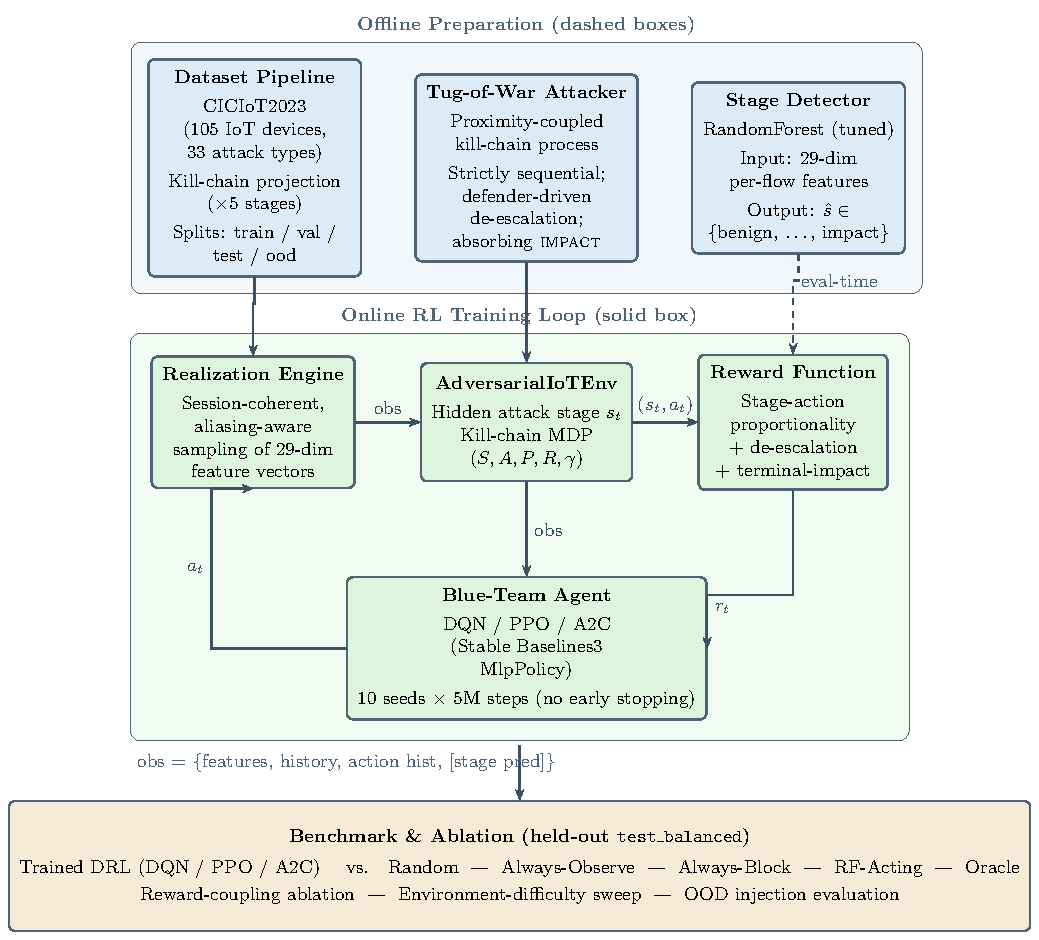
\includegraphics[width=\linewidth]{architecture_diagram.pdf}
\caption{Three-component pipeline: offline preparation, online RL training,
and held-out evaluation. The defender observes only aliased feature windows,
never the true kill-chain stage.}
\label{fig:architecture}
\end{figure}

\subsection{Data and kill-chain projection}
We use CICIoT2023~\cite{Neto2023}, collected from $105$ real IoT devices as
pre-aggregated flow records. We drop $17$ zero-variance/highly-correlated
columns, retaining $29$ features, and map the $34$ labels ($33$ attacks +
benign) to the five stages through a deterministic projection $\pi_{kc}$ (full
table in~\ref{app:mapping}). After reserving OOD classes, the training
pool contains $235{,}324$ rows. Each stage $s$ induces an empirical
per-stage feature distribution $p_{\text{data}}(\mathbf{x}\mid s)$. We build disjoint
\texttt{train}, \texttt{val\_balanced}, \texttt{test\_balanced}, and
\texttt{ood} splits (disjointness is asserted in the test suite). Ten attack
classes (at least two per non-benign stage) are held out entirely for OOD
evaluation: VulnerabilityScan, Recon-OSScan (recon);
XSS, SqlInjection (access); Mirai-udpplain,
DNS\_Spoofing (maneuver); and DDoS-HTTP\_Flood,
DoS-SYN\_Flood, DDoS-SlowLoris, DDoS-ACK\_Fragmentation
(impact).

\subsection{Reactive tug-of-war attacker}
\label{sec:attacker}
The attacker begins benign and initiates activity autonomously with onset
probability $p_{\text{onset}}=0.35$ into recon (and $p_{\text{onset-access}}
=0.10$ directly into access). Thereafter it reacts to the defender's applied
force through a signed proportionality rule on
$d_t = a_t - \mathrm{rec}(s_t)$, where $\mathrm{rec}(s)$ is the
stage-appropriate response and $a_t$ the action taken:
under-forced ($d_t\!\le\!-1$) it advances one stage with probability
$p_{\text{up}}^{\text{eff}}$; proportionate ($d_t\!=\!0$) it retreats
one stage with $p_{\text{down}}=0.90$ (raised to $0.98$ under
\textsc{isolate}); over-forced ($d_t\!\ge\!1$) it holds. Escalation
pressure is coupled to proximity to impact,
\begin{equation}
p_{\text{up}}^{\text{eff}} = p_{\text{up}}
\big(\sigma_{\min} + (1-\sigma_{\min})\,\lambda\big),
\label{eq:proximity}
\end{equation}
with $p_{\text{up}}=0.90$, residual floor $\sigma_{\min}=0.4$, and proximity
factor $\lambda = s/4$ for stage index $s\in\{0,\dots,4\}$, so the
attacker is harder to push back the closer it is to impact. An attack held
below impact for the full horizon yields a prevention bonus; a tie at the
impact boundary resolves in the attacker's favor.

\subsection{Partial observability and the aliasing knob}
\label{sec:pomdp}
The defense is a partially observable Markov decision process (POMDP)
$(\mathcal{S},\mathcal{A},\mathcal{O},P,Z,R,\gamma)$.
The defender never sees $s_t$; it receives a feature row through an
observation aliasing kernel that, with probability $\alpha$, emits a row
drawn from a stage adjacent to the true one:
\begin{equation}
Z(\mathbf{x}\mid s) = (1-\alpha)\,p_{\text{data}}(\mathbf{x}\mid s)
           + \alpha\,p_{\text{data}}(\mathbf{x}\mid s\pm 1).
\label{eq:aliasing}
\end{equation}
The rate $\alpha\in[0,1]$ is the central experimental knob: $\alpha=0$ is a
fully observable per-flow world (a classifier's best case), while larger
$\alpha$ forces temporal inference. The agent observes a stacked window
$\mathbf{o}_t = [\mathbf{x}_{t-4}, \Delta\mathbf{x}_{t-4}, \dots,
\mathbf{x}_t, \Delta\mathbf{x}_t]\in\mathbb{R}^{290}$
(window $w=5$ of $29$ features plus first differences), a finite-memory
surrogate for the belief state $b(s)$. The action set is
$\mathcal{A}=\{\textsc{observe}, \textsc{log}, \textsc{restrict},
\textsc{block}, \textsc{isolate}\}=\{0,1,2,3,4\}$. Episodes start benign, run
to $100$ steps with a lifecycle floor of $20$, and impact is non-terminal in
the primary reward function (the defender still gets one final decision turn).

\subsection{Stage detector and the memoryless baseline}
\label{sec:detector}
A tuned Random Forest ($200$ trees, max depth $20$, min-samples-leaf $2$,
balanced class weights; $\approx\!2.6$M parameters, $22$~MB) predicts the stage
from a single feature row, reaching a macro-$F_1$ of $\DetectorRfFoneBalanced$
on \texttt{test\_balanced} (grid search over $54$ cells,
validation macro-$F_1$ $0.927\pm0.005$). The deployable, memoryless
baseline --- \textbf{RF-Acting} --- maps each row to a predicted stage and then
to the recommended action. It is memoryless by construction: it sees one
row per decision, so the RL-vs-RF comparison isolates windowed temporal
control vs.\ memoryless control, not ``RL vs.\ supervised learning'' in the
abstract (a point we return to in Section~\ref{sec:discussion}).

\subsection{Reward functions}
\label{sec:reward}
A \texttt{reward\_mode} switch selects between two reward functions. The
\textbf{primary} function is \texttt{outcome} (sparse): only an action cost
$-\kappa\,C_{\text{action}}(a)$ ($\kappa=1$) and terminal accounting. At impact,
the penalty $-p_{\text{impact}}=-200$ always applies; a terminal
\textsc{block}/\textsc{isolate} adds $+b_{\text{success}}=+250$, a passive
\textsc{observe}/\textsc{log} adds $-p_{\text{missed}}=-150$, and
\textsc{restrict} adds $0$. A one-time prevention bonus
$+b_{\text{prevent}}=+50$ is granted if impact is averted for the full horizon.
The \textbf{coupled} function (used only in the reward-coupling
ablation) reinstates six stage-conditioned shaping terms: a proportionality
bonus ($+5$ if $|a-\mathrm{rec}|\!\le\!1$), a disproportionality penalty ($-5$
if $\ge\!2$), a benign-passivity bonus ($+10$), an over-reaction penalty
($-50$), and block guardrails ($-100$ on benign, $-50$ on recon), plus a
capped per-pushback de-escalation bonus ($+15$ each, cap $150$). All results
use \texttt{outcome} unless stated.

\subsection{Agents, baselines, and protocol}
\label{sec:protocol}
We train three independent Stable-Baselines3~\cite{Raffin2021} agents on a
Gymnasium environment~\cite{Gymnasium2023}, all with a $2\times64$ ReLU MLP
policy: DQN~\cite{Mnih2015} (off-policy value baseline), PPO~\cite{Schulman2017}
(on-policy actor-critic), and A2C~\cite{Mnih2016} (faster on-policy). Each is
trained for a fixed $5{,}000{,}000$ steps with no early stopping over
$\NumSeeds$ seeds $\{0,\dots,9\}$; the best-on-validation checkpoint is carried
forward. Evaluation uses $n=300$ episodes per policy. Baselines are: Random,
Always-observe, Always-block, RF-Acting (deployable memoryless controller;
Section~\ref{sec:detector}), and a Recommended-Action Oracle that reads
the true stage --- a non-competitor ceiling. We report bootstrap $95\%$
confidence intervals and treat non-overlapping intervals as separation. The
full hyperparameters are in Section~\ref{sec:hparams}.

\subsection{Hyperparameters}
\label{sec:hparams}
All agents use a $2\times64$ ReLU MLP policy.
\textbf{PPO}: lr $3\times10^{-4}$, $n_{\text{steps}}=2048$, $\gamma=0.99$,
$\lambda_{\text{GAE}}=0.95$, entropy $0.010$, value coef.\ $0.50$, batch $64$,
$10$ epochs. \textbf{A2C}: lr $7\times10^{-4}$, $n_{\text{steps}}=256$,
$\gamma=0.99$, $\lambda_{\text{GAE}}=0.95$, entropy $0.010$, value coef.\ $0.50$.
\textbf{DQN}: lr $5\times10^{-4}$, $\gamma=0.99$, batch $64$, buffer $200$k,
learning-starts $5000$, target-update $5000$, exploration fraction $0.20$
($1.0\!\to\!0.05$), max-grad-norm $0.5$.

% =====================================================================
\section{Results}
\label{sec:results}
% =====================================================================

All experiments run CPU-only (Python~3.9, PyTorch, scikit-learn, SB3,
Gymnasium), and the accompanying test suite reports $\NumTests$ passing tests.
Our tuned RF stage detector attains a macro-$F_1$ of $\DetectorRfFoneBalanced$,
with per-class $F_1$ from $0.87$ (recon/access) to $0.998$ (impact); its only
material confusion is recon$\to$access ($13.2\%$).

\subsection{The observation-aliasing crossover}
\label{sec:results-crossover}
Table~\ref{tab:alpha} and Fig.~\ref{fig:alpha} report mean episode reward
across the aliasing sweep. At $\alpha=0$ PPO ($\AlphaZeroPPO$) and RF
($\AlphaZeroRF$) tie (gap $\AlphaZeroGap$, overlapping CIs), where the gap is
defined as the PPO minus RF mean reward: the environment is not rigged for
RL --- in a fully observable per-flow world the memoryless classifier is as good
as the sequential policy. As $\alpha$ rises the classifier degrades
monotonically ($\AlphaZeroRF \to \AlphaTwoRF \to \AlphaFourRF \to \AlphaSixRF
\to \AlphaEightRF \to \AlphaOneRF$, i.e.\ net-harmful at full aliasing), while
windowed PPO stays essentially flat ($\AlphaFourPPO$ at the headline
$\alpha=\HeadlineAlpha$). The gap becomes significant (disjoint CIs)
from $\alpha=\HeadlineAlpha$ ($\AlphaFourGap$) and widens to $\AlphaOneGap$ at
$\alpha=1.0$. A2C is highest throughout (e.g.\ $\AlphaFourATwoC$ at headline),
and the oracle ceiling is $\OracleCeiling$.

\begin{table}[t]
\centering
\caption{Mean episode reward vs.\ aliasing rate $\alpha$ ($n=300$,
$95\%$ CI half-widths omitted for space; see Fig.~\ref{fig:alpha}).
``Gap'' is PPO$-$RF.}
\label{tab:alpha}
\small
\begin{tabular}{@{}lrrrrr@{}}
\toprule
$\alpha$ & PPO & A2C & DQN & RF & Gap \\
\midrule
0.0 & \AlphaZeroPPO  & \AlphaZeroATwoC  & \AlphaZeroDQN  & \AlphaZeroRF  & \AlphaZeroGap \\
0.2 & \AlphaTwoPPO   & \AlphaTwoATwoC   & \AlphaTwoDQN   & \AlphaTwoRF   & \AlphaTwoGap \\
0.4 & \AlphaFourPPO  & \AlphaFourATwoC  & \AlphaFourDQN  & \AlphaFourRF  & \AlphaFourGap \\
0.6 & \AlphaSixPPO   & \AlphaSixATwoC   & \AlphaSixDQN   & \AlphaSixRF   & \AlphaSixGap \\
0.8 & \AlphaEightPPO & \AlphaEightATwoC & \AlphaEightDQN & \AlphaEightRF & \AlphaEightGap \\
1.0 & \AlphaOnePPO   & \AlphaOneATwoC   & \AlphaOneDQN   & \AlphaOneRF   & \AlphaOneGap \\
\bottomrule
\end{tabular}
\end{table}

\begin{figure}[t]
\centering

\includegraphics[width=\linewidth]{Falpha_curve.pdf}
\caption{The crossover. The memoryless classifier (RF-Acting) degrades
monotonically with aliasing while windowed RL stays flat; the policies tie at
$\alpha=0$ and separate with disjoint CIs from $\alpha=\HeadlineAlpha$ onward.}
\label{fig:alpha}
\end{figure}

Structurally, RF-Acting fails as $\alpha$ grows because a misread row triggers
a mismatched action; the windowed agents instead integrate evidence over the
window and defer commitment. Benign false-positive rates stay below $1\%$ for
all RL agents (PPO $0.89\%$, DQN $0.46\%$, A2C $0.66\%$) versus $100\%$ for
always-block and $41.3\%$ for random.

\subsection{Reward-coupling ablation}
\label{sec:results-coupling}
A natural objection is that the RL advantage stems from a privileged shaped
reward. We retrain all agents under both reward functions at
$\alpha=\HeadlineAlpha$ (Fig.~\ref{fig:coupling}). The best RL agent beats
RF under both: under the coupled function the best agent (DQN,
$\CouplingDQNCoupled$) leads RF ($+163.1$), and under the sparse outcome
function the best agent (A2C, $\CouplingATwoCOutcome$) leads RF ($+83.1$); in
both cases the best-RL-minus-RF gap is about $+63$ in the RL agent's favor.
Shaping changes which algorithm wins and how reliably it trains, but not
the qualitative result that learned control beats the memoryless controller.

\begin{figure}[t]
\centering

\includegraphics[width=\linewidth]{Fcoupling_reward_gap.pdf}
\caption{Best-RL-minus-RF reward gap under the coupled (shaped) and outcome
(sparse) reward functions at $\alpha=\HeadlineAlpha$. The best RL agent leads RF
in both regimes.}
\label{fig:coupling}
\end{figure}

\subsection{Out-of-distribution prevention}
\label{sec:results-ood}
We stress the policies on ten held-out attack classes via single-stage feature
injection (held-out rows replace only their own stage's realization). The best
RL agent (A2C) prevents a fraction between $\FfifteenBestRLPreventionLow$ and
$\FfifteenBestRLPreventionHigh$ on every class, versus
$\FfifteenRFPreventionLow$--$\FfifteenRFPreventionHigh$ for RF; the per-class
advantage ranges $\FfifteenAdvantageLow$ to $\FfifteenAdvantageHigh$
(Fig.~\ref{fig:ood}). RF fails structurally: it spends roughly
two-thirds of steps in \textsc{observe}/\textsc{log}, lets the attacker reach
impact, and only mitigates the final turn --- ``mitigated,'' not
``prevented.''

Crucially, the RL advantage shows no detectable dependence on the
detector's per-class recall, which spans a graded spectrum from
$\FfifteenDNSSpoofingRecall$ (DNS\_Spoofing) through $\FfifteenVulnScanRecall$
(VulnerabilityScan) up to $\FfifteenSynFloodRecall$ (DoS-SYN\_Flood): the
Spearman correlation is $\rho=\FfifteenSpearmanRho$ ($p=\FfifteenSpearmanP$),
Pearson $r=\FfifteenPearsonR$ ($p=\FfifteenPearsonP$), and a bootstrap OLS
slope CI $[\FfifteenOLSSlopeCILow, \FfifteenOLSSlopeCIHigh]$ spans zero
(Fig.~\ref{fig:ood-recall}). We emphasize this is a no-detectable-trend
finding at $n=10$ classes, not proven independence; the primary evidence is the
direct per-class dominance, which holds even for the highest-recall classes.

\begin{figure*}[t]
\centering
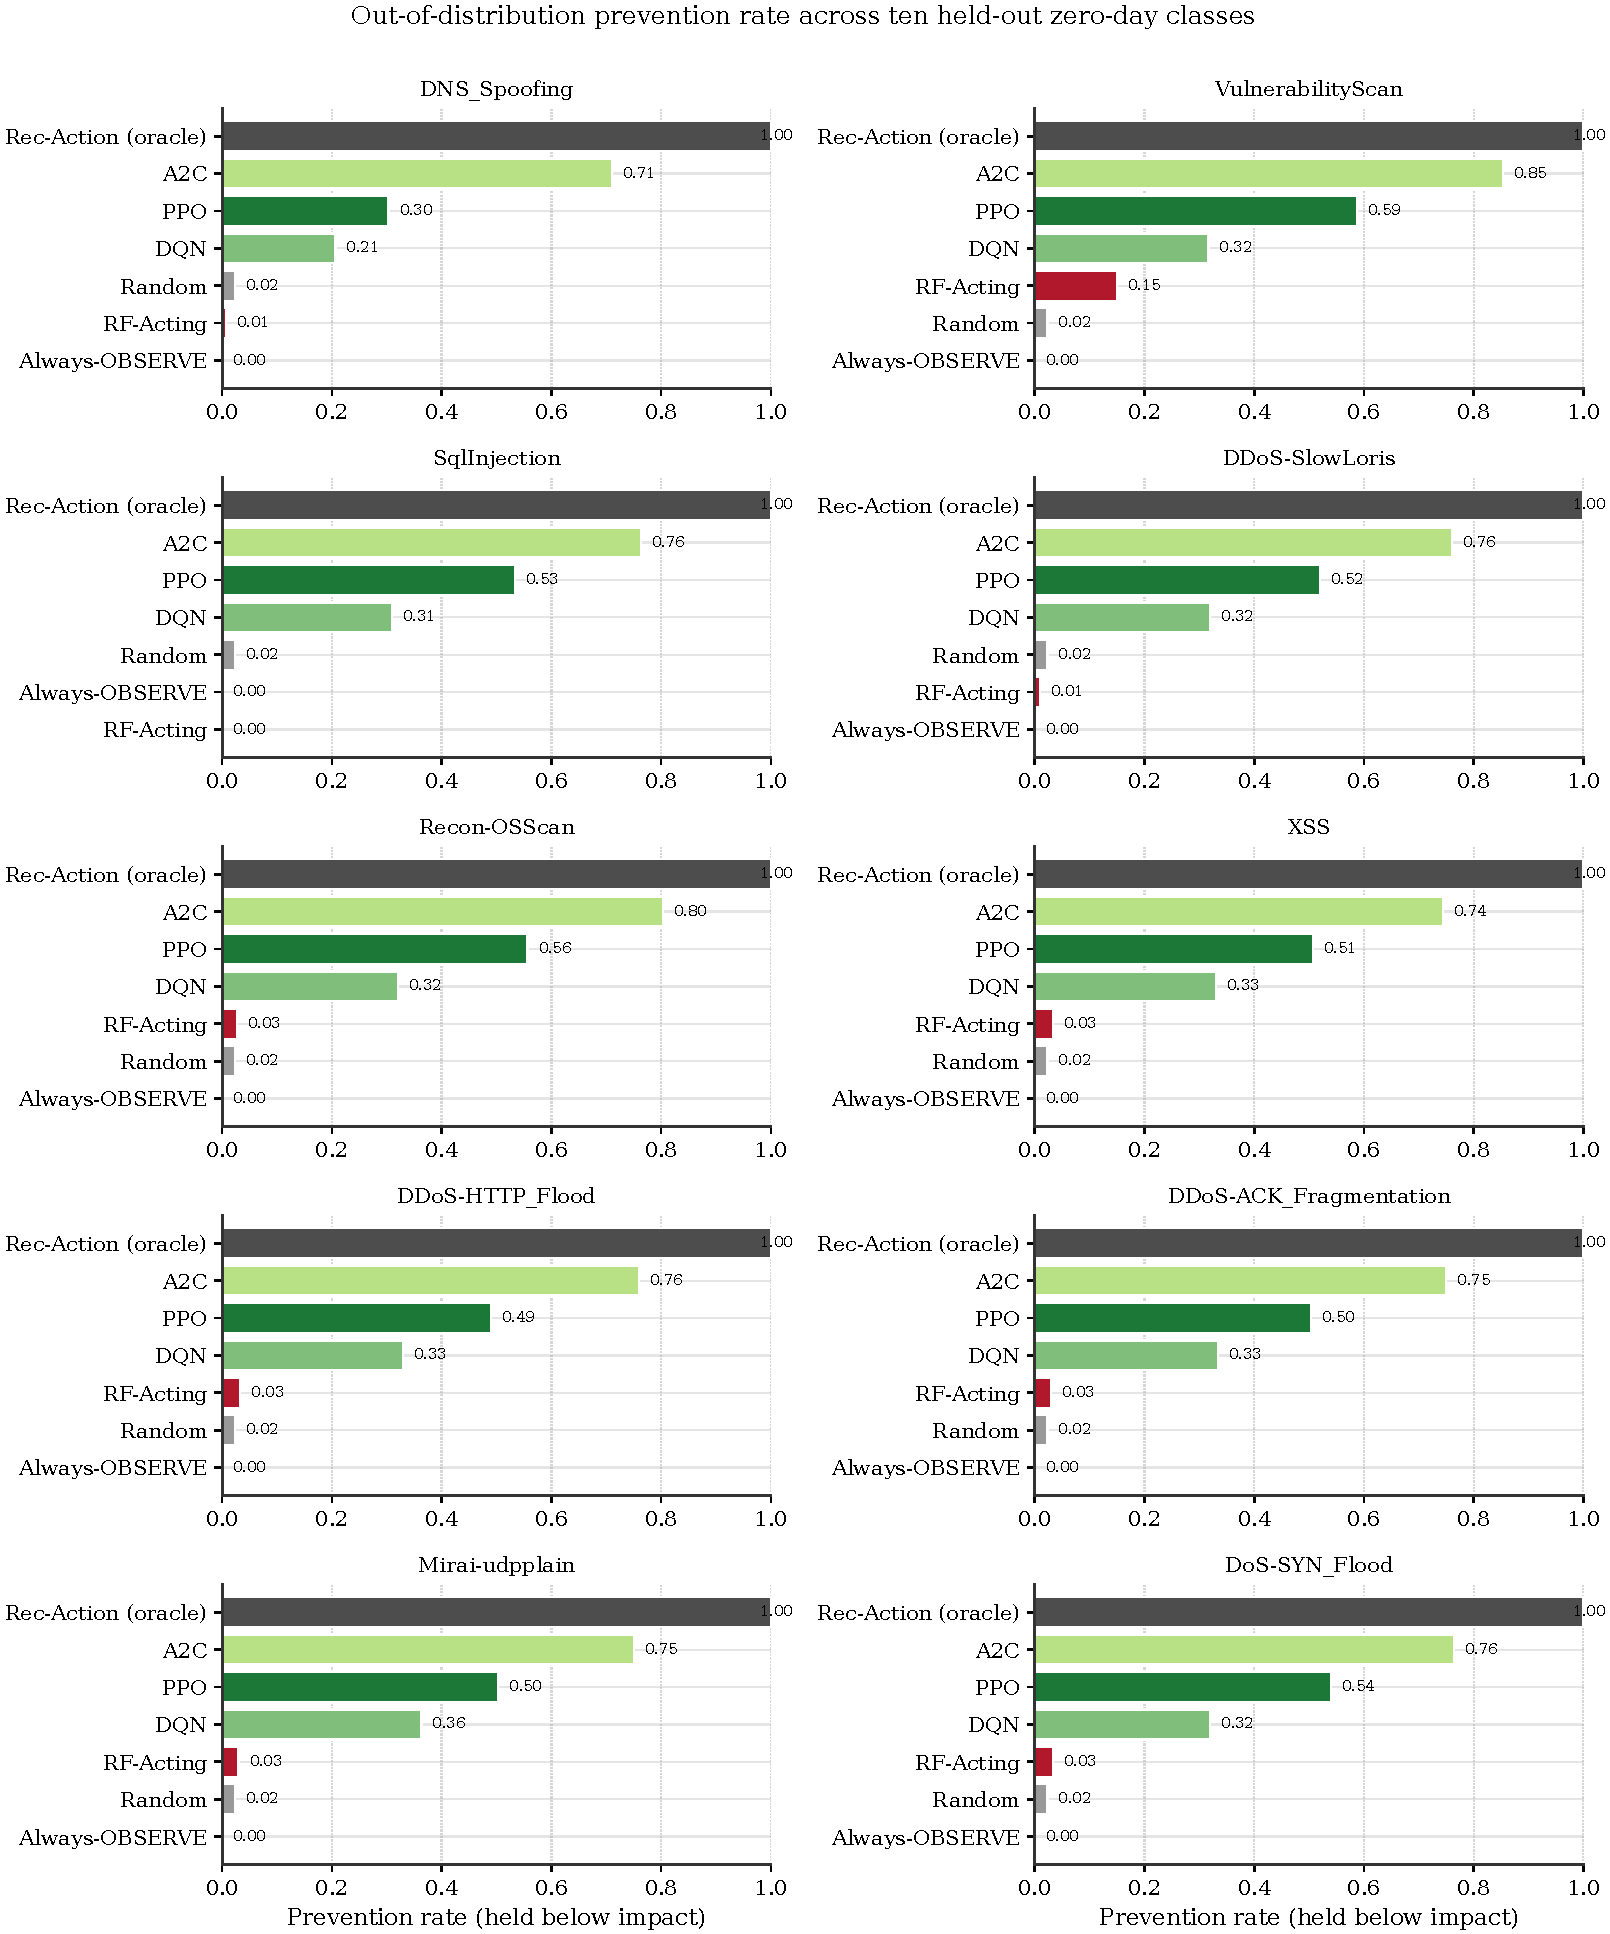
\includegraphics[width=\textwidth]{F15_ood_robustness.pdf}
\caption{Per-class prevention on ten held-out classes: best RL prevents
$\FfifteenBestRLPreventionLow$--$\FfifteenBestRLPreventionHigh$ everywhere;
RF prevents $\FfifteenRFPreventionLow$--$\FfifteenRFPreventionHigh$.}
\label{fig:ood}
\end{figure*}

\begin{figure}[t]
\centering
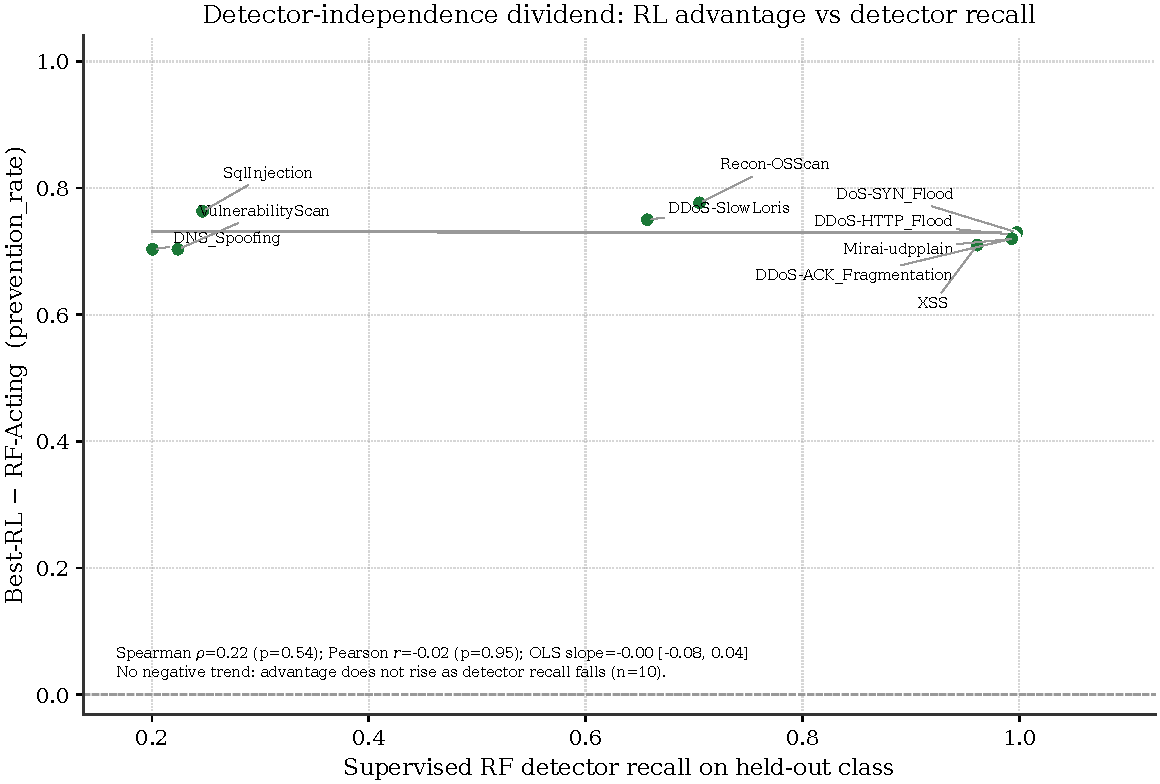
\includegraphics[width=\linewidth]{F15b_recall_vs_advantage.pdf}
\caption{RL-minus-RF prevention advantage vs.\ detector per-class recall.
No detectable trend ($\rho=\FfifteenSpearmanRho$, OLS slope CI spans zero).}
\label{fig:ood-recall}
\end{figure}

\subsection{Training reliability and learned doctrines}
\label{sec:results-reliability}
Both on-policy agents lock onto stable plateaus above the RF band within
$\approx0.2$M steps, with low across-seed standard deviation (PPO $\approx15$,
A2C $\approx9$), while DQN shows wide bands throughout ($\approx52$ under the
outcome function, tightening to $\approx17$ under coupled shaping)
(Fig.~\ref{fig:learning}). The on-policy advantage is thus one of
training-time stability, not peak return: the same DQN that wins the
coupled ablation ($\CouplingDQNCoupled$) collapses to $\CouplingDQNOutcome$
under the sparse outcome reward.

The agents learn distinct doctrines (Fig.~\ref{fig:actions}): A2C is
\emph{prevent-at-maneuver}, blocking $86.5\%$ of maneuver-stage steps and never
isolating; PPO is \emph{contain-at-impact}, isolating at impact ($12.1\%$);
DQN is flatter and more observation-heavy. These are qualitatively different,
defensible policies rather than a single ``optimal'' response.

\begin{figure}[t]
\centering

\includegraphics[width=\linewidth]{F3_learning_curves.pdf}
\caption{Learning curves ($\NumSeeds$ seeds). On-policy agents converge to
tight bands above RF; DQN bands stay wide under the sparse reward.}
\label{fig:learning}
\end{figure}

\begin{figure}[t]
\centering

\includegraphics[width=\linewidth]{F4_action_distribution.pdf}
\caption{Per-stage action distributions revealing distinct doctrines:
A2C prevents at maneuver; PPO contains at impact.}
\label{fig:actions}
\end{figure}

\subsection{Robustness sweeps}
\label{sec:results-sweeps}
Re-evaluating the fixed headline PPO across an environment-difficulty sweep
(attacker retreat probability $p_{\text{down}}\in\{0,\dots,1\}$) yields a
monotone ordering A2C $>$ PPO $>$ DQN, with the widest RL margin at the harshest
setting (Fig.~\ref{fig:aggressiveness}). Under an evasive-persistence
(post-detection hardening) sweep (Fig.~\ref{fig:evasion}), degradation is
graceful: A2C declines from
$\FseventeenZeroATwoCReward$ to $\FseventeenSeventyFiveATwoCReward$ and PPO from
$\FseventeenZeroPPOReward$ to $\FseventeenSeventyFivePPOReward$; A2C passes and
PPO narrowly fails the pre-registered $25\%$-degradation gate (CI-low
degradation $\FseventeenPPOCILowDegradation$).

% =====================================================================
\section{Discussion and threats to validity}
\label{sec:discussion}
% =====================================================================

We state the limitations that bound our claims.

\textbf{(1) Designed, non-co-adaptive attacker.} The crossover is
conditional on this attacker class. A qualitatively different or
co-adaptive adversary could shrink or erase the gap; self-play is deferred to
future work.

\textbf{(2) Aliasing and session coherence are modeling abstractions.}
CICIoT2023 flows are pre-aggregated with no recoverable session key, so
$\alpha$ and session coherence are imposed at the environment layer. Our
contribution is the shape of the response as $\alpha$ varies, anchored
by the $\alpha=0$ tie rather than by any single absolute number.

\textbf{(3) The supervised baseline is memoryless by construction.} The
comparison therefore isolates windowed temporal control vs.\ memoryless
control, not ``RL vs.\ supervised learning'' in general. A windowed supervised
controller (e.g.\ an HMM or a TCN/LSTM head plus the recommended-action rule,
over the same window) is the single most direct strengthening and our foremost
follow-up. The reward-coupling ablation and the $\alpha=0$ tie already rule out
the two strongest alternative explanations (privileged reward; an
RL-favoring environment).

\textbf{(4) Single dataset.} We use CICIoT2023 only; Bot-IoT~\cite{Koroniotis2019}
is the named replication target. The OOD study is a controlled feature-injection
stress test, not a claim of deployed zero-day generalization.

\textbf{(5) Statistical power of the recall-independence claim.} With $n=10$
held-out classes, the near-zero recall--advantage correlation is
``no detectable trend,'' not proven independence; the load-bearing evidence is
the direct per-class dominance.

% =====================================================================
\section{Conclusion}
\label{sec:conclusion}
% =====================================================================

We framed autonomous IoT defense as a partially observable, kill-chain-aware
control problem and asked when a learned sequential policy beats a
memoryless classifier. Three findings answer it: (i) the two tie in a fully
observable world and diverge as observation aliasing grows, with the classifier
becoming net-harmful while windowed RL stays flat; (ii) the best RL agent beats
the classifier under both sparse and shaped rewards; and (iii) RL prevents more
attacks on every held-out class with no detectable dependence on detector
recall. On-policy methods buy training-time stability rather than higher peak
return. Future directions include recurrent belief-state policies (a
preliminary recurrent-PPO run did not beat the windowed feed-forward
policy under our budget), non-monotonic and co-adaptive attackers, train-time
OOD augmentation, edge-hardware deployment ($\approx20$~KB policy footprint),
multi-agent self-play, federated multi-site training, and a constrained-MDP
formulation for a hard false-positive ceiling.

% =====================================================================
\appendix
\section{Reproducibility protocol}
\label{app:repro}
Every figure ships a sibling \texttt{manifest.json} recording input SHA-256
hashes, the git commit, and the producing script. A fresh checkout reproduces
the suite with \texttt{pytest -q} ($\NumTests$ passing) and verifies the hash
chain with \texttt{python -m scripts.reproducibility\_smoke} (verdict
\textsc{pass}). Full retraining is available through documented pipeline
targets. Hardware is CPU-only (Python~3.9, PyTorch-CPU, scikit-learn, SB3,
Gymnasium).

\section{Label-to-stage mapping}
\label{app:mapping}
The deterministic map $\pi_{kc}$ assigns each of the $34$ CICIoT2023 labels to
one of the five kill-chain stages: \textsc{benign}: BenignTraffic;
\textsc{recon}: Recon-PortScan, Recon-OSScan, Recon-HostDiscovery,
Recon-PingSweep, VulnerabilityScan; \textsc{access}: SqlInjection,
CommandInjection, XSS, Backdoor\_Malware, BrowserHijacking, Uploading\_Attack,
DictionaryBruteForce; \textsc{maneuver}: MITM-ArpSpoofing, DNS\_Spoofing,
Mirai-greeth\_flood, Mirai-greip\_flood, Mirai-udpplain; \textsc{impact}: the
remaining DDoS/DoS flood, fragmentation, and SlowLoris labels. The ten OOD
classes (Section~\ref{sec:results-ood}) are held out entirely from training.

\section{Robustness-sweep figures}
\label{app:sweeps}
\setcounter{figure}{0}
\renewcommand{\theHfigure}{C.\arabic{figure}}
Figure~\ref{fig:aggressiveness} shows the environment-difficulty sweep over the
attacker retreat probability $p_{\text{down}}$, and Fig.~\ref{fig:evasion}
shows the evasive-persistence sweep; both are discussed in
Section~\ref{sec:results-sweeps}.

\begin{figure}[t]
\centering

\includegraphics[width=\linewidth]{F10_aggressiveness.pdf}
\caption{Environment-difficulty sweep over the attacker retreat probability
$p_{\text{down}}$. The RL ordering A2C $>$ PPO $>$ DQN is preserved throughout,
with the widest margin at the harshest setting ($p_{\text{down}}=0$).}
\label{fig:aggressiveness}
\end{figure}

\begin{figure}[t]
\centering

\includegraphics[width=\linewidth]{F17_evasion_sweep.pdf}
\caption{Evasive-persistence (post-detection hardening) sweep. Degradation is
graceful for all agents; A2C passes and PPO narrowly fails the pre-registered
$25\%$-degradation gate.}
\label{fig:evasion}
\end{figure}

% =====================================================================
\section*{Declaration of generative AI and AI-assisted technologies in the
manuscript preparation process}
% =====================================================================
During the preparation of this work the authors used a generative
AI assistant to help condense and copy-edit prose derived from the first
author's dissertation. After using this tool, the authors reviewed and edited
the content as needed and take full responsibility for the content of the
publication.

% =====================================================================
\section*{CRediT authorship contribution statement}
% =====================================================================
\textbf{Felipe Santos}: Conceptualization, Methodology,
Software, Investigation, Formal analysis, Data curation, Writing --- original
draft, Visualization. \textbf{Denis Fantinato}: Conceptualization,
Supervision, Methodology, Writing --- review \& editing, Project
administration.

% =====================================================================
\section*{Declaration of competing interest}
% =====================================================================
The authors declare that they have no known competing financial interests or
personal relationships that could have appeared to influence the work reported
in this paper.

% =====================================================================
\section*{Funding}
% =====================================================================
This research did not receive any specific grant from funding agencies in the
public, commercial, or not-for-profit sectors.

% =====================================================================
\section*{Data availability}
% =====================================================================
The raw CICIoT2023 dataset~\cite{CICIoT2023Dataset} is distributed under the
Canadian Institute for Cybersecurity license and is available from the original
providers; we therefore do not redistribute it. All code, processing
pipelines, trained-policy checkpoints, and the hash-chained result manifests
needed to reproduce every figure and number in this paper are archived at
\url{https://doi.org/10.5281/zenodo.XXXXXXX} (placeholder; replace before
submission) and mirrored at \url{https://github.com/feli-santos/rl-iot-defense-system}.

% =====================================================================
\section*{Acknowledgements}
% =====================================================================
The authors thank the members of the examining committee for their feedback on
the dissertation from which this work is derived.

% =====================================================================
\bibliographystyle{elsarticle-num}
\bibliography{refs}

\end{document}
